\documentclass[tikz,border=10pt]{standalone}
\usetikzlibrary{calc,angles,quotes,intersections}

\begin{document}
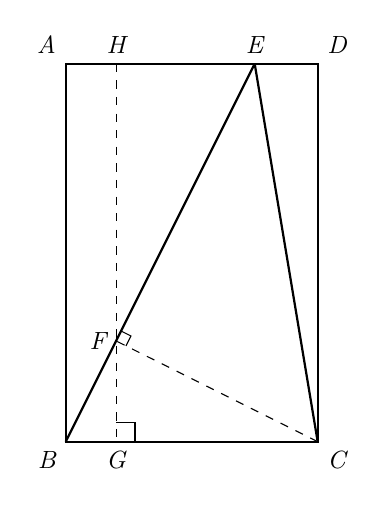
\begin{tikzpicture}[
    scale=0.8, 
    important line/.style={thick},
    dashed line/.style={dashed, thin},
    every node/.style={font=\small\itshape}
]

    % 1. 定义矩形四个顶点的坐标 (设定 A 为原点，宽5 高6)
    \coordinate (A) at (0,6);
    \coordinate (B) at (0,0);
    \coordinate (C) at (4,0);
    \coordinate (D) at (4,6);
    \coordinate (E) at (3,6); % 点 E 在 AD 上

    % 2. 绘制矩形轮廓
    \draw[important line] (A) -- (B) -- (C) -- (D) -- cycle;

    % 3. 绘制三角形 BCE 的实线边
    \draw[important line] (B) -- (E);
    \draw[important line] (E) -- (C);

    % 4. 计算点 F：满足 CF 垂直于 BE (点 F 在 BE 上)
    % 几何原理：点 F 是从 C 到直线 BE 的投影点
    \coordinate (F) at ($(B)!(C)!(E)$);

    % 5. 处理垂线 HG
    % H 在 AD 上，G 在 BC 上，且 HG 过 F 且与 BC 垂直
    \coordinate (G) at ($(B)!(F)!(C)$);
    \coordinate (H) at ($(A)!(F)!(D)$);

    % 6. 绘制虚线辅助线 (HG 和 CF)
    \draw[dashed line] (H) -- (G);
    \draw[dashed line] (C) -- (F);

    % 7. 绘制直角符号
    % G 处的直角（保留原有）
    \draw ($(G)+(0.3,0)$)--($(G)+(0.3,0.3)$)--($(G)+(0,0.3)$);
    
    % 核心新增：F 点处 CF⊥BE 的垂直标注（直角符号）
    % 方法1：用 angles 库的直角标注（更规范，推荐）
    \pic[draw, angle radius=4pt] at (F) {right angle = C--F--E};
    
    % 方法2（备选）：手动绘制直角符号（与G点风格统一）
    % \pgfmathsetmacro{\rot}{atan2(\y{E}-\y{B},\x{E}-\x{B}) - 90}
    % \begin{scope}[rotate around={\rot:(F)}]
    %   \draw ($(F)+(-0.2, -0.2)$)--($(F)+(-0.2,0)$)--($(F)+(0,-0.2)$);
    % \end{scope}

    % 8. 标注文字标签 (使用 auto 计算位置以避免压线)
    \node[above left] at (A) {A};
    \node[below left] at (B) {B};
    \node[below right] at (C) {C};
    \node[above right] at (D) {D};
    \node[above] at (E) {E};
    \node[left] at (F) {F};
    \node[below] at (G) {G};
    \node[above] at (H) {H};

\end{tikzpicture}
\end{document}